\documentclass[sigconf]{acmart}
% defining the \BibTeX command - from Oren Patashnik's original BibTeX documentation.
\def\BibTeX{{\rm B\kern-.05em{\sc i\kern-.025em b}\kern-.08emT\kern-.1667em\lower.7ex\hbox{E}\kern-.125emX}}
% Remove the annoying stuff
\settopmatter{printacmref=false} % Removes citation information below abstract
\renewcommand\footnotetextcopyrightpermission[1]{} % removes footnote with conference information in first column
\pagestyle{plain} % removes running headers



\usepackage{Nikolai}





\begin{document}

%
% The "title" command has an optional parameter, allowing the author to define a "short title" to be used in page headers.
\title{CMIS Hand-in 4: Finite Element Method}

\author{Nikolai Plambech Nielsen}
\email{lpk331@alumni.ku.dk}
\affiliation{%
  \institution{Niels Bohr Institute, University of Copenhagen}
}


\maketitle

\section{The Finite Element Method}
The essence of the finite element method is to represent the domain as a finite set of elements (hence the name), and compute an approximate solution for each of these elements, adding up to the global solution. The actual elements vary on the dimensionality of the system. Straight-line segments for 1D problems, triangles for 2D and tetrahedra for 3D are the ones we focus on here due to their simplicity, but others can be used as well.

The actual method can be summarised in a series of steps:
\begin{enumerate}
	\item Convert the differential equation to a volume integral
	\item Define the elements
	\item Choose a shape and trial function for the elements
	\item Compute the elementwise integrals
	\item Assemble the global matrix and source vector
	\item Apply boundary conditions
	\item Compute the solution
\end{enumerate}
In this hand-in we focus on implementing the method in 1D and 2D, and use it to solve the Poisson equation for a simple source term:
\begin{equation}\label{key}
	\grad^2 u = c
\end{equation}
where to begin with we set $ c=0 $, and later $ c\in \mathbb{R} $, subject to point-wise boundary conditions $ u(\V{r}) = a(\V{r}) , \forall \V{r} \in \Gamma $.

\paragraph{Step 1.} In the first step of the recipe we multiply each side by a function $ v(\V{r}) $, which must be continuously differentiable and 0 on the boundary of the domain ($ v(\V{r})=0,\ \forall \ \V{r}\in \Gamma $). Then we integrate over the domain on both sides to get
\begin{equation}\label{key}
	\int_{\Omega} v(\V{r}) \grad^2 u(\V{r}) \ud \Omega = \int_{\Omega} v(\V{r}) c \ud x
\end{equation}
This formulation of the problem is still equivalent to the original form, and is called ``Strong Form''. Next we perform integration by parts on the left hand side:
\begin{equation}\label{key}
	\int_{\Omega} v(\V{r}) \grad^2 u(\V{r}) \ud \Omega = \int_{\Gamma} v(\V{r}) \grad u(\V{r}) \ud \Gamma - \int_{\Omega} \grad v(\V{r}) \grad u(\V{r}) \ud \Omega
\end{equation}
But the first term is zero by definition, leading to the ``Weak Form'' of the problem:
\begin{equation}\label{key}
\int_{\Omega} \grad v(\V{r}) \grad u(\V{r}) \ud \Omega =- \int_{\Omega} v(\V{r}) c \ud \Omega
\end{equation}
This takes care of the first step. 

\paragraph{Step 2.} In the second step we use the methods from last weeks hand-in on the generation of computational meshes. In particular I define the geometry of the setup in a \texttt{.poly} file and relegate the mesh generation to the \texttt{Triangle} program written by J. R. Shewchuk.

\paragraph{Step 3.} For the third step we approximate the unknown $ u $ by the function
\begin{equation}\label{key}
	u \approx \sum_{e\in \Omega} \V{N}^e \hat{u}^e,
\end{equation}
where the sum runs over all elements in the system, $ \hat{u}^e $ is a vector of the value of $ u $ on the 3 vertices in the $ e $'th element (with vertices counted counter clockwise): $ \hat{u}^e  = [u_i^e \ u^e_j \ u^e_k]^T $, and $ \V{N}^e $ is the ``shape function'' for the element. The shape function must have the following properties
\begin{equation}\label{key}
	N_i(\V{r}) = \begin{cases}
	1 & \V{r} = \V{r}_i, \\ 0, & \V{r}_j \land j \neq i
	\end{cases}, \quad \sum_{i} N_i(\V{r}) = 1.
\end{equation}
The first ensures proper interpolation for the points, whilst the second ensures that the approximation of $ \V{u} $ is exact on all vertices in the system. In one dimension we use a hat-function:
\begin{equation}\label{key}
	N_i(x) = \max\pp{0, 1- \vv{\frac{x_i - x}{\Delta x}}}
\end{equation}
which are 1 on the $ i $'th vertex, and 0 on all other (assuming equal spacing of nodes in the domain $ \Delta x $). And for triangles in two dimensions we use barycentric coordinates:
\begin{equation}\label{key}
	N_i^e(\V{r}) = \frac{A_i^e}{A^e}
\end{equation}
where the geometry is as seen in figure \ref{fig:barycentric}.
\begin{figure}
	\centering
	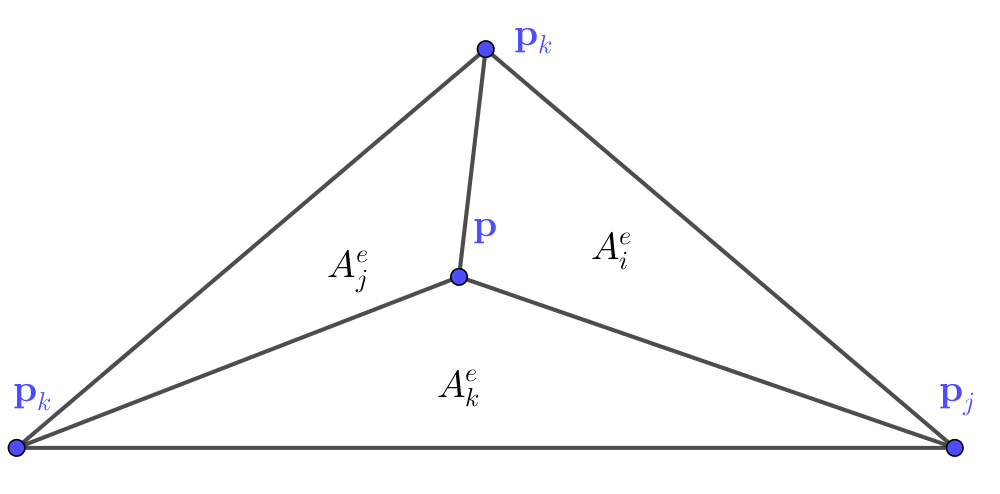
\includegraphics[width=0.7\linewidth]{barycentric.png}
	\caption{Barycentric coordinates for a triangular element.}
	\label{fig:barycentric}
\end{figure}
Where the areas can be found as the magnitudes of cross products:
\begin{equation}\label{key}
	N_i^e = \frac{\vv{(\V{p}_k - \V{p}_j) \times (\V{p}-\V{p}_j)}}{2 A^e}, \quad A^e = \frac{1}{2} \vv{(\V{p}_j - \V{p}_i) \times (\V{p}_k - \V{p}_i)}
\end{equation}
Now, the points of the triangles are two dimensional, so the cross products are also just the determinant of the $ 2 \times 2 $ matrix $ [(\V{p}_k - \V{p}_j),  \ (\V{p}-\V{p}_j) $ and equivalently for the total area, and other barycentric coordinates.

We also need the spatial derivatives of the shape functions, which in one dimension, for the straight line between nodes $ i $ and $ j $ gives
\begin{equation}\label{key}
	\diff{N_i^e}{x} = \frac{-1}{\Delta x}, \quad \diff{N^e_j}{x} = \frac{1}{\Delta x}
\end{equation}
And in two dimensions
\begin{equation}\label{key}
	\diff{N_i^e}{x} = -\frac{p_{k,y} - p_{j,y}}{2A^e}, \quad \diff{N_i^e}{y} = \frac{p_{k,x} - p_{j,x}}{2 A^e}
\end{equation}
All of which are independent of the free variable $ \V{r} $.

Next we choose the trial function to be $ v(\V{r}) = \V{N}(\V{r}) \delta \V{u} $, where $ \delta \V{u} $ is a vector of arbitrary values (a choice reminiscent of the techniques used in the principle of least action). Substituting the shape and trial functions into the volume integral gives
\begin{equation}\label{key}
	\int_{\Omega} \grad (\V{N}(\V{r}) \delta \V{u}) \grad \V{N}(\V{r}) \hat{u} \ud \Omega =- \int_{\Omega} (\V{N}(\V{r})\delta \V{u}) c \ud \Omega
\end{equation}
or utilizing $ v(\V{r})^T = v(\V{r}) $ since $ v $ is a scalar and contracting the integral
\begin{equation}\label{key}
\delta \V{u}^T \int_{\Omega} \grad \V{N}^T(\V{r}) \grad \V{N}(\V{r}) \hat{u} + \V{N}^T(\V{r}) c \ud \Omega = 0 
\end{equation}
Since this must hold for all choices of $ \delta \V{u} $, the integral itself must be zero. We can then manipulate the integral further to get a linear set of equations for $ \hat{u} $:
\begin{equation}\label{key}
\bb{\int_{\Omega} \grad \V{N}^T(\V{r}) \grad \V{N}(\V{r}) \ud \Omega}  \hat{u} = -c \int_{\Omega} \V{N}^T(\V{r}) \ud \Omega, \quad \V{K}\hat{u} = \V{f}
\end{equation}
where $ \V{K} $ is the left hand side integral, and $ \V{f} $ is the right hand side integral. Next we split up the integral in the individual elements:
\begin{equation}\label{key}
	\V{K} = \int_{\Omega} \grad \V{N}^T(\V{r}) \grad \V{N}(\V{r}) \ud \Omega = \sum_{e\in \Omega} \int_{\Omega^e} \grad (\V{N}^e)^T \grad \V{N}^e \ud \Omega = \sum_{e\in \Omega} \V{K}^e.
\end{equation}
and likewise for the source vector. Really, the individual element matrices are $ N \times N $, where $ N $ is the number of vertices in the domain, but only 9/4 elements are non-zero, so we just calculate a $ 3\times 3 $ ($ 2\times 2 $) matrix, and add the values in the right place of $ \V{K} $.


\paragraph{Step 4.} In both one and two dimensions all integrands are independent of the integration variables, and we just get an extra factor of $ A^e $ (which is $ \Delta x $ for one dimension), along with an outer product between a vector and itself:
\begin{equation}\label{key}
	\int_{\Omega^e} \diff{(\V{N}^e)^T}{x} \diff{\V{N}^e}{x} \hat{u}^e \ud \Omega = A^e \diff{(\V{N}^e)^T}{x} \diff{\V{N}^e}{x} \hat{u}^e
\end{equation}
The source term is 
\begin{equation}\label{key}
	\V{f}^e = -\int_{\Omega^e} (\V{N}^e)^T c \ud \Omega
\end{equation}
If $ c = 0 $ then we trivially have $ \V{f}^e = 0 $. if instead, $ c \neq 0 $ we get (in two dimensions):
\begin{equation}\label{key}
	f^e_i = -\frac{cA^e}{3}
\end{equation}
which can be seen by integrating any of the barycentric coordinates over a triangle with points $ \V{p}_i = (0,0), \V{p}_j = (\alpha, 0), \V{p}_k = (\beta, \gamma) $. Any triangle can be rotated and translated to have these coordinates if we let $ 0 < \alpha \leq \beta $, meaning the result is general.

In one dimension we get from straight integration.
\begin{equation}\label{key}
	f^e_i = \Delta x / 2
\end{equation}



\paragraph{Step 5.} Next we need to put all the different element matrices into the global matrix. Here we can leverage the fact since the element matrices consists of an outer product between one vector and itself, the resulting matrices are symmetric. This means we do not have to worry too much about the index order when assembling the system. For each element we take the global index of the vertices in the element, create a meshgrid of these values, and add the 9/4 (2D/1D) values in the element matrix to the corresponding values in the global matrix. Note the adding part: since each vertex may be represented in a multitude of elements, we need to incorporate the contribution from all elements.

The source vector is built similarly, except for each element there are only 3/2 elements to add.

\paragraph{Step 6.}
Since we are dealing with point-wise / Dirichlet bondary conditions, incorporating these amounts to just clamping the values on the vertices to be the boundary condition value. This means that we just set the row of the $ n $'th element to 0, except for the $ n $'th entry, which we set to a one. We also set the $ n $'th entry in the source term equal to the value of the boundary condition, leading to the equation:
\begin{equation}\label{key}
	\hat{u}_n = a(\V{p}_n)
\end{equation}

\paragraph{Step 7.} Last we just need to solve the linear system of equations. If the system is not uniquely defined (ie, the matrix rank is non-singular) without the boundary conditions, then hopefully by adding these we get a full-rank matrix, and we can employ a direct solver. If not we resort to an iterative method. In our case (both one and two dimensions), our system is uniquely defined and we do indeed get a full-rank, non-singular matrix.

\section{Experiments}
For this weeks experiments we solve the system on a rectangular domain with $ x \in [0, 6] $ and $ y \in [0, 2] $, subject to the boundary condition $ u(0, y) = a, \ u(6, y) = b $.

To evaluate the accuracy of the method, we compare the numerical solution $ \hat{u}_i $ to the analytical solution $ u(\V{p}_i) $ using the root mean square:
\begin{equation}\label{key}
	\text{res} = \sqrt{\sum_{i} (\hat{u}_i - u(\V{p}_i))^2/N_{\text{dof}}}
\end{equation}
where $ N_{\text{dof}} $ is the number of degrees of freedom for the system - ie the total number of nodes in the domain, minus the number of nodes subject to boundary conditions. (this ensures we get a nonsensical result in degenerate cases, like ones where all nodes are boundary nodes).

\subsection{The analytical solution}
In the case of $ c\in \mathbb{R} $ we can solve the system analytically. With these boundary conditions we exclude all dependence on $ y $, giving an analytical solution (found by integrating a constant twice, and solving for two known points to get the factors of the linear and constant term):
\begin{equation}\label{key}
	u(x, y) = \frac{c}{2}x^2 - \frac{18c + a - b}{6} x + a
\end{equation}
which also includes the straight line solution of $ c=0 $:
\begin{equation}\label{key}
	u(x,y) = \frac{b-a}{6} x + a = \frac{\Delta y}{\Delta x} x + a
\end{equation}

\subsection{One dimension}
In one dimension the $ \V{K} $ matrix only has elements along the main and two off diagonals, since each vertex is only part of two neighbouring elements. Because of this, the matrix is equal to what one would get if one uses the finite difference method, without ghost nodes, and using dirichlet boundary conditions. Letting $ c=0 $ and solving for a computational mesh of 11 equidistant points between 1 and 2 gives the result seen in figure \textbf{REF}. The solution is just $ u = x $, and we see that the residual is but an order of magnitude above the machine epsilon, even with just 11 points.

I suspect this is not because of some insane precision in the finite element method, but rather due to the fact, that the shape functions are essentially a piecewise linear interpolation between points, so when the solution \textit{is} a linear function, it will be as close to exact as possible.

Indeed we will see this as we go to the two dimensional case, and set $ c\neq 0 $

\end{document}
